\documentclass[10pt,a4article]{amsart}
\usepackage{amsfonts}
\usepackage{amsthm}
\usepackage[ruled,vlined]{algorithm2e}
\usepackage{amsmath}
\usepackage{amscd}
\usepackage[latin2]{inputenc}
\usepackage{t1enc}
\usepackage[mathscr]{eucal}
\usepackage{indentfirst}
\usepackage{graphicx}
\usepackage{graphics}
\usepackage{pict2e}
\usepackage{epic}
\numberwithin{equation}{section}
\usepackage[margin=2.9cm]{geometry}
\usepackage{epstopdf}
\usepackage{amsmath,amsthm,verbatim,amssymb,amsfonts,amscd, graphicx}
\usepackage{mathtools}
\usepackage[dvipsnames]{xcolor}

 

\usepackage[backend=bibtex,firstinits=true,style=alphabetic,maxbibnames=9,natbib=true,url=false,sorting=nyt,doi=true,backref=false]{biblatex}
%\usepackage[backend=bibtex,firstinits=true,style=alphabetic,natbib=true,maxcitenames=2,maxbibnames=10,url=false,doi=true,backref=false]{biblatex}
\addbibresource{sb.bib}
\renewbibmacro{in:}{\ifentrytype{article}{}{\printtext{\bibstring{in}\intitlepunct}}}
\renewcommand*{\bibfont}{\small}

\DeclareMathOperator{\sgn}{sgn}

\newcommand{\note}[1]{{\leavevmode\color{BrickRed}{#1}}}

 
\usepackage[colorlinks,linkcolor = red, citecolor=blue]{hyperref} 

 
\definecolor{mypink1}{rgb}{0.858, 0.188, 0.478}
\definecolor{mypink2}{RGB}{219, 48, 122}
\definecolor{mypink3}{cmyk}{0, 0.7808, 0.4429, 0.1412}
\definecolor{mygray}{gray}{0.6}


% For aligned \stackrel, use \leftstackrel
\newlength{\leftstackrelawd}
\newlength{\leftstackrelbwd}
\def\leftstackrel#1#2{\settowidth{\leftstackrelawd}%
{${{}^{#1}}$}\settowidth{\leftstackrelbwd}{$#2$}%
\addtolength{\leftstackrelawd}{-\leftstackrelbwd}%
\leavevmode\ifthenelse{\lengthtest{\leftstackrelawd>0pt}}%
{\kern-.5\leftstackrelawd}{}\mathrel{\mathop{#2}\limits^{#1}}}

 
\theoremstyle{plain}
\newtheorem{Th}{Theorem}
\newtheorem{Lemma}[Th]{Lemma}
\newtheorem{Cor}[Th]{Corollary}
\newtheorem{Prop}[Th]{Proposition}

 \theoremstyle{definition}
\newtheorem{Def}[Th]{Definition}
\newtheorem{Conj}[Th]{Conjecture}
\newtheorem{Rem}[Th]{Remark}
\newtheorem{?}[Th]{Problem}
\newtheorem{Ex}[Th]{Example}

\newcommand{\im}{\operatorname{im}}
\newcommand{\Hom}{{\rm{Hom}}}
\newcommand{\diam}{{\rm{diam}}}
\newcommand{\ovl}{\overline}

\def\R{{\mathbb R}}
\def\Q{{\mathbb Q}}
\def\Z{{\mathbb Z}}
\def\N{{\mathbb N}}
\def\C{{\mathbb C}}
\def\E{{\mathbb E}}
\def\R{{\mathbb R}}
\def\Y{{\mathcal Y}}
\def\L{{\mathcal L}}
\def\H{{\mathcal H}}
\def\D{{\mathcal D}}
\def\P{{\mathbb P}}
\def\M{{\mathbb M}}
\def\V{{\mathcal V}}
\def\S{{\mathbb S}}
\def\A{{\mathbf A}}
\def\x{{\mathbf x}}
\def\b{{\mathbf b}}
\def\a{{\mathbf a}}
\def\Ph{{\mathbf {\Phi}}}

\def\h{{\mathbf{h}}}
\def\G{{\Gamma}}
\def\s{{\sigma}}
\def\e{{\varepsilon}}
\def\l{{\lambda}}
\def\p{{\phi}}
\def\v{{\mathbf{v}}}
\def\t{{\theta}}
\def\z{{\zeta}}
\def\o{{\omega}}
\def\y{{\mathbf{y}}}
\def\g{{\mathbf{g}}}
\def\u{{\mathbf{u}}}
\def\w{{\mathbf{w}}}



\begin{document}

\title{\textbf{A brief introduction to stochastic bandits}}
\date{}
\author{Yiming Xu}
\maketitle


\section{Set-up and algorithms}

The note provides a brief introduction to the fundamentals of stochastic bandit learning. Particularly, we introduce the set-up of the problem as well as a few related algorithms. The discussion is based on the chapters $6$-$10$ and $13$-$16$ in \cite{lattimore2018bandit}.

Suppose that you are facing a $k$-armed slot machine. Every time you can choose one arm to play and the corresponding reward will be revealed to you immediately. Rewards of the arms not played in the round are assumed hidden. In the context of stochastic bandits, rewards generated by each arm are iid random variables. One may think bandits in this case being neutral. Suppose you will play $n$ rounds in total. The goal of bandit learning, roughly speaking, is to find a policy under which the regret is asymptotically as small as possible. Even though the rigorous definitions of a policy as well as the regret are yet to be articulated, it can be felt that a good policy should strike a balance between exploration of the underplayed arms and exploitation of the well-played arms giving high rewards on average. The rule of thumb, as we will see, is to be slightly optimistic when faced with uncertainty. 

Let $A=[k]$ be the set of arms and $n$ be the \emph{horizon} of the game. $\{x_{ti}\}_{t\in [n]}$ denote the sequential rewards generated by arm $i$ in $n$ rounds, which are iid random variables with distribution $\nu_i$ and mean $\mu_i$. Here we assume that $\nu_i$ are $1$-\emph{subgaussian} and \emph{unstructured}, in the sense that acquiring knowledge on one arm imply nothing about the others. A counterexample to this is $\mu_2=1-\mu_1$ when $k\geq 2$. A \emph{deterministic policy} is defined as $\pi = (\pi_t)_{t\in [n]}\in [k]^n$ such that $\pi_t$ is a measurable function of $\{x_{t'\pi_{t'}}\}_{t'\in [t-1]}$. A \emph{non-deterministic policy}, on the other hand, possesses extra randomness conditional on the outcomes observed in the past.  We will mainly focus on the deterministic strategies in the study of stochastic bandits. Intuitively, this means that which arm to play in round $t$ is determined by the information disclosed before $t$. The \emph{regret} $R_n(\pi)$ of $\pi$ is defined as the average difference between rewards collected under $\pi$ and the best possible arm:
\begin{align}
R_n(\pi):=\max_{i\in [k]}\E\left[\sum_{t\in [n]}(x_{ti}-x_{t\pi_t})\right]=\max_{i\in [k]}\mu_i -\E\left[\sum_{t\in [n]}x_{t\pi_t}\right]. \label{s:1}
\end{align}
The randomness within the expectation comes from $\{x_{ti}\}_{i\in [k], t\in [n]}$ (and $\pi$ if $\pi$ is non-deterministic).  

A few things to note. Whether regret defined in \eqref{s:1} is meaningful needs further clarification. Also, it is not clear what kind of bounds would imply that a policy $\pi$ is good. The first question is hard to justify from a mathematical point of view. We may consider \eqref{s:1} as a good place to start with when studying stochastic bandits.  For the second question, note that if using the trivial policy by selecting a fixed arm, one would expect a regret which is linear in $n$.  Therefore, any policy achieving sublinear regret would be reasonable, and how far this can go is the topic we will explore later.

In the following analysis, without loss of generality we assume that arm $1$ is optimal. For $i\in [k]$, define the \emph{suboptimality gap} between $i$ and $1$ as $\Delta_i=\mu_1-\mu_i$. For any $t\leq n$, define the total number of rounds where $i$ is chosen before $t$ under policy $\pi$ as $T_i(t; \pi)$, which is a random quantity adapted to the natural filtration. Using the tower property of expectation, one can rewrite $R_n(\pi)$ as 
\begin{align}
R_n(\pi)=\sum_{i\in [k]}\Delta_i\E[T_i(n; \pi)].\label{s:2}
\end{align} 
Such form provides a convenient way to analyze $R_n$.  Indeed, since the summation is over $i$, one often only needs to bound $\E[T_i(n; \pi)]$ for each $i$ under a given policy.  

We mention two well-known algorithms in stochastic bandit learning: The Explore-then-Commit (ETC) algorithm and the Upper Confidence Bound (UCB) algorithm, each of which is followed by a short summary of their pros and cons, as well as some asymptotic regret results.   


\begin{algorithm}
\DontPrintSemicolon
 \KwIn{$m$: number of exploration on each arm.}
 \KwOut{ $\pi=(\pi_t)_{t\in [n]}$}
 \While{$t\leq km$}{
\begin{align*}
\pi_t &=  \lceil t\bmod {k}\rceil\\
t &= t +1.
\end{align*}}
\While{$km<t\leq n$}{
\begin{align*}
\pi_t = \arg\max_{i\in [k]}\frac{1}{m}\sum_{t = 1}^{mk}x_{t\pi_t}\mathbb{I}\{\pi_t = i\}
\end{align*}
}
\caption{The Explore-then-Commit Algorithm. } 
\label{alg:ETC}
\end{algorithm}

The idea behind Algorithm \ref{alg:ETC} is simple. Divide $n$ rounds into two parts: first $mk$ rounds for equal exploration on each arm and the remaining time for exploitation on the arm demonstrating the best performance. One must settle for a trade-off between these two. If $m$ is small, there is a considerable chance that exploration is poor, resulting in the exploitation procedure sub-optimal.  If $m$ is large, the regret generated in the exploration process will likely dominate. Therefore, the best $m$ is usually set at some middle point, as summarized in the following theorem. 

\begin{Th}\label{thm:ETC}
The regret $R_n$ under ETC is given by
\begin{align}
R_n\leq m\sum_{i\in [k]}\Delta_i + (n-mk)\sum_{i\in [k]}\Delta_i e^{-m\Delta_i^2/4}.
\end{align}
Particularly, when $k=2$, taking $m=\max\left\{1, 4\Delta_2^{-2}\log(n\Delta_2^2/4)\right\}$ yields
\begin{align}
R_n\leq\Delta_2+C\sqrt{n},\label{ETC:opt}
\end{align}
where $C$ is some absolute constant. 
\end{Th}

Theorem \ref{thm:ETC} follows from a direct application of concentration inequalities. There are a few things worth remarking here. Firstly, a high-probability version of the result on the \emph{psedo-regret} $\bar{R}_n$ (which is defined as the conditional expectation on the policy) can be obtained similarly:
\begin{align*}
\P\left(\bar{R}_n:=n\mu_1-\sum_{t\in [n]}\mu_{\pi_t}\leq m\sum_{i\in [k]}\Delta_i\right)\geq 1-\sum_{i\in [k]}e^{-m\Delta_i^2/4}. 
\end{align*} 
Secondly, despite the fact that \eqref{ETC:opt} gives an optimal bound on regret (which will be specified later), how to achieve it depends on knowledge of both the suboptimality gaps $\Delta_i$ and the horizon $n$. These quantities are usually fixed but may not be revealed to the player in advance. In theory, it can be shown that for two-armed bandits the dependence on $\Delta_i$ can be removed while obtaining a sub-optimal regret bound $n^{2/3}$, and the dependence on $n$ can be resolved by a doubling trick without increasing the regret two much. To address the dependence on the sub-optimal gaps, another algorithm called UCB has been proposed, see Algorithm \ref{alg:UCB}. 

\begin{algorithm}
\DontPrintSemicolon
 \KwIn{$\delta$: confidence level.}
 \KwOut{ $\pi=(\pi_t)_{t\in [n]}$}
 \While{$t\leq n$}{
\begin{align*}
\pi_t = \arg\max_{i\in [k]}\text{UCB}_i(t-1, \delta),
\end{align*}
where for $i\in [k]$,
\begin{align*}
\text{UCB}_i(t-1, \delta) =\begin{cases} 
      \infty & T_i(t-1)=0 \\
       \displaystyle\frac{1}{T_i(t-1)}\sum_{s\in [t-1]}x_{s\pi_s}\mathbb{I}\{\pi_s = i\}+\sqrt{\frac{2\log(1/\delta)}{T_i(t-1)}} & T_i(t-1)>0 \\
   \end{cases}
\end{align*}}
\caption{The Upper Confidence Bound Algorithm. } 
\label{alg:UCB}
\end{algorithm}
Break ties equally if there are more than one maximizer. Algorithm \ref{alg:UCB} first explores all arms exactly once, then estimates each arm using the (sample-mean based) upper bound of its $\delta$-confidence interval obtained from the Hoeffding inequality. Intuitively, the arm chosen in round $t$ either has a large sample mean or is underexplored compared to other arms. A suboptimal arm is unlikely to be played long since its optimism bonus is decreasing to zero. The key ingredient lies in choosing a good confidence level $\delta$, which again balances the trade-off between exploration and exploitation.  
\begin{Th}\label{thm:UCB}
Set $\delta=n^{-2}$. The regret under UCB is given by
\begin{align*}
R_n\leq 3\sum_{i=1}^k\Delta_i +\sum_{i: \Delta_i>0}\frac{16\log n}{\Delta_i}.
\end{align*}
\end{Th}
\begin{proof}
Let $c\in (0,1)$ be a fixed number. Consider the intersection of two events: a. UCB overestimates arm $1$ at least once in $n$ rounds; b. UCB for each suboptimal arm $i$ falls below $\mu_1$ at time $t_i$, where $t_i$ is chosen such that $(1-c)\Delta_i\geq\sqrt{2\log(1/\delta)/t_i}$. It is easy to check that this intersected event occurs with probability at least $1-n\delta-\sum_{i: \Delta_i>0}e^{-t_ic^2\Delta^2_i/2}$. Applying the total probability formula, one obtains an upper bound for $R_n$ using the decomposition form \eqref{s:1}:
\begin{align*}
R_n\leq n\left(n\delta+\sum_{i: \Delta_i>0}e^{-t_ic^2\Delta^2_i/2}\right)+\sum_{i\in [k]}\Delta_i t_i.
\end{align*}
Setting $\delta=n^{-2}$ and $c=1/2$ yields the desired result.   
\end{proof}
Theorem \ref{thm:UCB} may seem loose when $\Delta_i$ are small. To settle this issue, separate the  arms into two parts: those with sub-optimality gap less than $\sqrt{16k\log n/n}$ and greater than $\sqrt{16k\log n/n}$. Bounding $\E[T_i(n)]$ by $n$ in the first part and by Theorem \ref{thm:UCB} in the second gives
\begin{align}
R_n\leq 3\sum_{i\in [k]}\Delta_i + 8\sqrt{nk\log n}. \label{bdd:UCB}
\end{align} 
The regret in Theorem \ref{thm:UCB} differs only by a log factor compared to the optimal bound by ETC. Yet it does not require knowledge on the suboptimality gaps. This gains UCB popularity in many practical situations. Still, there are a few things we could consider for extension. First of all, the confidence level in Theorem \ref{thm:UCB} depends on horizon. This can be removed by choosing $\delta$ in a decreasing format, say, $\delta_t = (1+t\log^2 t)^{-1}$, and the resulting bound on regret remains unchanged (even better from simulation results). Secondly, when calculating the UCB, the Hoeffding inequality is used, which can be rather loose sometimes. For example, consider the Bernoulli bandits whose means are close to $0$ or $1$. In such situations, one could apply the Chernoff bound instead, which gives a confidence interval based on relative entropy. The corresponding regret will be improved by a taming factor (which usually depends on variance). Also, UCB works without the subgaussian assumption on rewards. One could replace the sample mean estimator by the median-of-means estimator in defining UCB. For any distributions whose second moment exists, the regret is similar to what we have in Theorem \ref{thm:UCB} but with a worse constant factor. 

We would like to mention that the $\log n$ factor in \eqref{bdd:UCB} can be removed by making the confidence level arm-dependent. This is achieved in an algorithm termed Minimax Optimal Strategy in the Stochastic case, or MOSS.  As the name suggests, this algorithm achieves asymptotic optimality under the minimax criteria. Precisely, for arm $i$ in round $t$,  MOSS selects $\delta_{t, i}=\min\{1, (kT_i(t-1)/n)^2\}$. One can show that regret in this case satisfies
\begin{align*}
R_n\leq 38\sqrt{kn}+\sum_{i\in [k]}\Delta_i. 
\end{align*}
This is of the same order as the best possible minimax lower bound for stochastic bandits. However, the hidden cost is that that the variance of the pseudo-regret increases significantly. More details will be given on this in the future study. 

Another algorithm called $\e$-Greedy is also built upon the philosophy of being optimistic is good. Instead of estimating via upper confidence bounds in the case of UCB, it takes a non-deterministic policy that forces exploration on arms which look sub-optimal. The details are given below:
\begin{algorithm}
\DontPrintSemicolon
 \KwIn{$(\e_t)_{t\in [n]}$: exploration parameters.}
 \KwOut{ $\pi=(\pi_t)_{t\in [n]}$}
 \While{$t\leq k$}{\begin{align*}
 \pi_t = t
 \end{align*}}
 \While{$k<t\leq n$}{
\begin{align*}
\pi_t \sim\begin{cases}
 \displaystyle\arg\max_{i\in [k]}\left\{\frac{1}{T_i(t-1)}\sum_{s\in [s-1]}x_{si}\mathbb{I}\{\pi_t = i\}\right\}\ \ \ \text{with probability}\ 1-\e_t\\
 \text{Uniform}([k])\ \ \ \text{with probability}\  \e_t
 \end{cases}
\end{align*}}
\caption{The $\e$-Greedy Algorithm. } 
\label{alg:e-greedy}
\end{algorithm}

Note that as $t$ becomes large, the time spent on exploration should diminish in order to get a good regret bound. Indeed, if choosing $\e_t\geq \e$ as a constant for all $t\in [n]$, one would expect 
\begin{align*}
\lim_{n\rightarrow\infty}\frac{R_n}{n} = \frac{\e}{k}\sum_{i\in [k]}\Delta_i. 
\end{align*}
By carefully choosing $\e_t$ as a decreasing function of $t$, we can get some comparable results as before:
\begin{Th}\label{thm:e-greedy}
Let $\Delta=\min_{i: \Delta_i>0}\Delta_i$ and $\e_t = \min\{1, Ct^{-1}\Delta^{-2}k\}$, where $C$ is some sufficiently large constant. Then, the regret under the $\e$-Greedy satisfies
\begin{align*}
R_n\leq C'\sum_{i\in [k]}\left(\Delta_i+\frac{\Delta_i}{\Delta^2}\log\left\{e, \frac{n\Delta^2}{k}\right\}\right),
\end{align*}
where $C'$ is an absolute constant. 
\end{Th}

Theorem \ref{thm:e-greedy} gives a similar bound to the one in Theorem \ref{thm:ETC} and \ref{thm:UCB}. The choice for $\e$, which is horizon-independent, requires only information on the smallest suboptimality gap. However, the unspecified constant $C$ may make the performance of the algorithm uncertain in practice.  

Before proceeding further to discuss the lower bounds on regret, we give some numerical simulations to verify the bounds derived so far. The bandit in the following experiment is set as $2$-armed Gaussian with horizon $n=1000$. The suboptimality gap $\Delta$ is chosen in $10$ different levels: $[1:10]*10^{-1}$.  Algorithms including ETC ($m=20, 50, 80$ as well as the close-to-optimal choice $\max\left\{1, 4\Delta_2^{-2}\log(n\Delta_2^2/4)\right\}$), UCB, UCB with horizon-free confidence levels, MOSS and $\e$-Greedy ($C=0.2$) are tested. For fixed $\Delta$, the regret $R_n$ for each policy is calculated by averaging over $1000$ independent samples. The results are in Figure \ref{fig:1}. 
\begin{figure}
  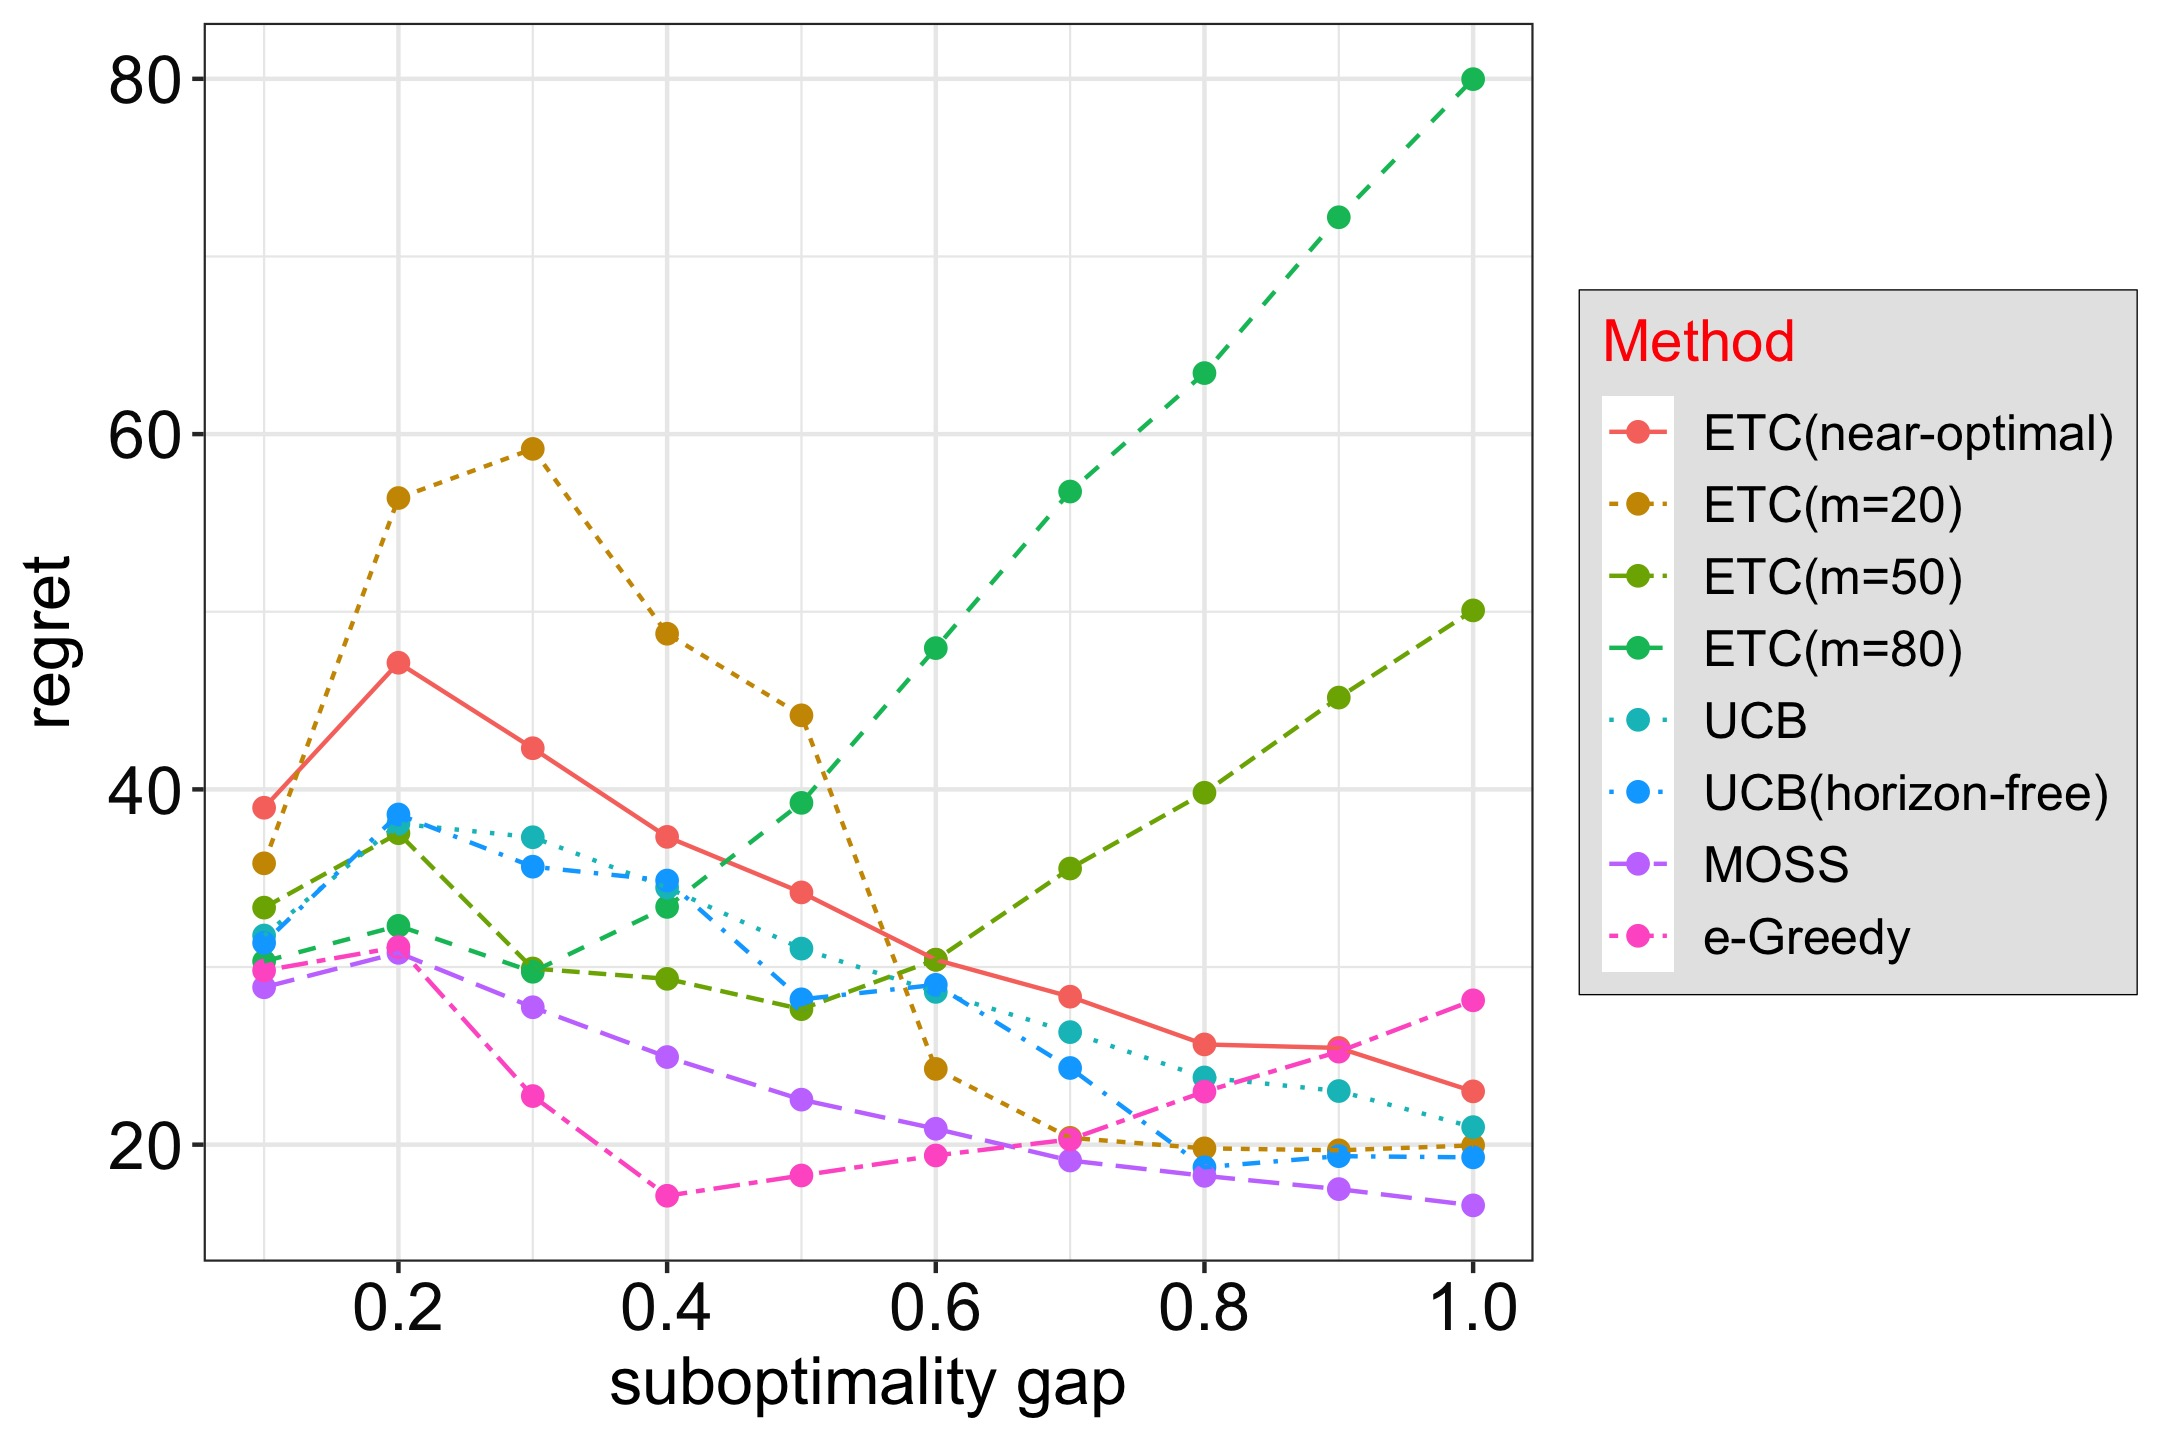
\includegraphics[width=12cm]{sb}
  \caption{Numerical simulations of several stochastic learning policies for two-armed Gaussian bandits with varying suboptimality gap.}
  \label{fig:1}
\end{figure}





\section{Lower bounds on regret}

To see how good the regret bounds derived in Algorithm \ref{alg:ETC} and \ref{alg:UCB}, we introduce the \emph{minimax} lower bound to quantify the comparison. Let $\V$ be the environment class, or equivalently, the set of admissible distributions on rewards: $\otimes_{i\in [k]}\nu_i$. The worst-case regret for a policy $\pi$ is defined as 
\begin{align*}
R_n(\pi, \V):=\sup_{\otimes_{i\in [k]}\nu_i\in\V}R_n(\pi).
\end{align*}
The minimax regret $R_n^*$ is the best worst-case regret among all possible policies $\Pi$: 
\begin{align}
R_n^*:=\inf_{\pi\in\Pi}R_n(\pi, \V).\label{s:mm}
\end{align}
Obtaining lower bounds on \eqref{s:mm} helps us understand the limitation of stochastic bandit learning. We introduce a natural way to approach this problem.  The general idea is to show that for any $\pi\in\Pi$, there exist two environments $\nu, \nu'\in\V$ such that $R_{n,\nu}(\pi)$ and $R_{n,\nu'}(\pi)$ cannot be small at the same time. Intuitively, a good instance for $\nu$ is bad for $\nu'$, and vice versa. If $\V$ is a parametrization family, this implies that the parameter of $\nu$ is distant from the parameter of $\nu'$. On the other hand, the difference between $\nu$ and $\nu'$ can be reflected in the difference between $R_{n,\nu}(\pi)$ and $R_{n,\nu'}(\pi)$ if $\pi$ sees $\nu$ and $\nu'$ similarly, which means that $\nu$ and $\nu'$ should not be too far away from each other. The right construction of $\nu$ and $\nu'$ is therefore relying on finding a trade-off point.  
\begin{Th}\label{s:minimax}
Let $\V$ be the class of normalized Gaussian bandits with their mean $\mu=(\mu_i)_{i\in [k]}\in [0,1]^k$. Suppose that the horizon $n\geq k-1$. Then for any policy $\pi$ there exists some $\nu\in\V$ such that
\begin{align}
R_{n,\nu}(\pi)\geq\frac{1}{27}\sqrt{(k-1)n}. \label{s:6}
\end{align}  
\end{Th}
\begin{proof}
Fix a policy $\pi$. Let $\Delta\in [0, 1/2]$ be some parameter to be tuned later. Consider two bandits as follows:
\begin{align*}
\nu &= (\Delta, 0, \cdots, 0)\\
\nu' &= (\Delta, \cdots, 2\Delta, 0, \cdots, 0),
\end{align*}
where $\nu'$ differs from $\nu$ only on the $i$-th component, with $i$ being the arm which $\pi$ plays least often on average in $\nu$: $i=\arg\min_{j>1}\E_\nu[T_j(n)]$. It is clear that spending too much time on arm $1$ is good for $\nu$ but bad for $\nu'$. Precisely, using the decomposition form \eqref{s:2},
\begin{align}
R_{n, \nu}(\pi)+R_{n, \nu'}(\pi)\geq \frac{n\Delta}{2}\left(\P_\nu\left(T_1(n)\leq \frac{n}{2}\right)+\P_{\nu'}\left(T_1(n)> \frac{n}{2}\right)\right).\label{s:3}
\end{align}
The right-hand side of \eqref{s:3} can be bounded via Le Cam's method in statistics. A convenient form is to use the Bretagnolle-Huber inequality, which states that for probability measure $\P$ and $\Q$ on the same probability space $(\Omega, \mathcal{F})$, and $A\in\mathcal{F}$, 
\begin{align}
\P(A)+\Q(A^c)\geq\frac{1}{2}\max\left\{e^{-D(\P, \Q)}, e^{-D(\Q, \P)}\right\},\label{s:4}
\end{align}
where $D(\cdot, \cdot)$ is the relative entropy, with the latter argument being the reference measure. Let $A = \{T_1(n)\leq n/2\}$, and $\P, \Q$ be the $\pi$-induced measure on $([k]\oplus\R)^n$ under $\nu$ and $\nu'$, respectively. It can be checked by definition that 
\begin{align}
D(\P, \Q)& = \sum_{j\in [k]}\E_\nu[T_j(n)]D(\mu_j, \mu'_j)\label{s:5}\\
& = \E_\nu[T_i(n)]D(\mu_i, \mu'_i)\nonumber\\
& \leq\frac{2n}{k-1}\Delta^2\nonumber,
\end{align}
where the last inequality follows from the fact that $\sum_{j\in [k]}\E_\nu[T_i(n)]=n$. Plugging \eqref{s:4} and \eqref{s:5} into \eqref{s:3} yields
\begin{align*}
R_{n, \nu}(\pi)+R_{n, \nu'}(\pi)\geq\frac{n\Delta}{4}e^{-\frac{2n\Delta^2}{k-1}}. 
\end{align*}
Taking $\Delta = \sqrt{\frac{k-1}{4n}}$ gives the desired result. 
\end{proof}
The constant $1/27$ in the bound \eqref{s:6} can be improved to $1/8$ via a different approach, which considers a sequence of environment instead of two, that are mutually inconsistent. The rest of the proof goes similarly by using the Pinsker's inequality.   

Theorem \ref{s:minimax} may be conservative if one is only interested in lower bounds on a set of `good' policies. In this case, one may derive a stronger result on the asymptotic behaviour of the regret appealing to \emph{instance-dependent} analysis, which is presented as follows.  

First of all, let us clarify what the good policies are. A policy $\pi$ is \emph{consistent} over $\V$ if for all $\nu\in\V$ and $p>0$, 
\begin{align*}
\lim_{n\rightarrow\infty}\frac{R_{n, \nu}(\pi)}{n^p} = 0. 
\end{align*}
Roughly speaking, the regret of a consistency policy is of logarithmic order asymptotically. Denote by $\Pi_{c}(\V)$ the set of consistent policies over $\V$. The following theorem implies that such intuition is accurate in a strong sense. 

\begin{Th}\label{s:ins}
Let $\V = \otimes_{i\in [k]} \V_i$ and $1$ be the optimal arm. For any $\pi\in\Pi_c(\V)$,
\begin{align}
\liminf_{n\rightarrow\infty}\frac{R_n}{\log n}\geq \sum_{i: \Delta_i>0}\frac{\Delta_i}{d_{\inf} (\mu_i, \mu_1, \V_i)}, 
\end{align}
where $d_{\inf} (\mu_i, \mu_1, \V_i) = \inf_{\nu_i'\in\V_i, \mu(\nu)>\mu_1}D(\nu_i, \nu_i')$. 
\end{Th}
\begin{proof}
The idea of the proof is similar to Theorem \ref{s:minimax}. Note that \eqref{s:2} implies that it suffices to prove that for $i\in [k]$ with nonzero suboptimality gap, 
\begin{align*}
\E_\nu[T_i(n)]\geq d^{-1}_{\inf} (\mu_i, \mu_1, \V_i).
\end{align*}
To show this, consider a modified environment $\nu'$ that agrees with $\nu$ except at the $i$-th arm, which is equal to $\nu_i'\in\V_i$ such that $D(\nu_i, \nu_i') < d_{\inf} (\mu_i, \mu_1, \V_i)+\e$ for some $\e>0$. Applying the Bretagnolle-Huber inequality with $A = \{T_i(n)\leq n/2\}$ and $\P, \Q$ the $\pi$-induced measure on $([k]\oplus\R)^n$ under $\nu$ and $\nu'$, respectively, 
\begin{align}
R_{n, \nu}(\pi)+R_{n, \nu'}(\pi)\geq\frac{n}{2}\min\{\Delta_i, \mu(\nu_i')-\mu_1\}e^{-(d_{\inf} (\mu_i, \mu_1, \V_i)+\e)\E_\nu[T_i(n)]}.\label{s:7}
\end{align}
The left-hand side of \eqref{s:7} can be further bounded from above since $\pi$ is consistent. Indeed, for any $p>0$, there exists an absolute constant $c_p$ such that $R_{n, \nu}(\pi)+R_{n, \nu'}(\pi)<c_pn^p$. Plugging this in \eqref{s:7} and taking $n$, $\e$ and $p$ to $\infty$, $0$ and $0$, respectively in order, produces the desired result. 
\end{proof}
Theorem \ref{s:ins} is more of theoretical interest, as the asymptotic result often hides the worrying constants that matter in practice. However, from this point of view, it can be checked that MOSS is asymptotically optimal in the $1$-subgaussian environment.   


 
 
\end{document}